%%%%%%%%%%%%%%%%%%%%%%%%%%%%%%%%%%%%%%%%%%%%%%%%%%%%%%%%%%%%%%%%%
%%%  ISWC 2016 Demo:   %%%%
%%%%%%%%%%%%%%%%%%%%%%%%%%%%%%%%%%%%%%%%%%%%%%%%%%%%%%%%%%%%%%%%%

\documentclass[runningheads,a4paper]{llncs}
\usepackage{graphicx}
\usepackage{amsmath}
\usepackage{todonotes}
\usepackage{hyperref}
\usepackage{amssymb, bm}
\usepackage{indentfirst}

%%%%%%%%%%%%%%%%%%%%%%%%%%%%%%%
%%%  Beginning of document  %%%
%%%%%%%%%%%%%%%%%%%%%%%%%%%%%%%

\begin{document}

\title{A title}

\titlerunning{A title}

\author{Manel Achichi$^1$, Pasquale Lisena$^2$, Eva Fern\'{a}ndez$^2$, Wafa Bouneb$^2$, \\ Konstantin Todorov$^1$, Rapha\"{e}l Troncy$^2$}
\authorrunning{Achichi \textit{et al.}}
\institute{$^1$University of Montpellier, France\\ $^2$EURECOM, Sophia Antipolis, France}

\maketitle

%%%%%%%%%%%%%%%%%%
%%%  Abstract  %%%
%%%%%%%%%%%%%%%%%%

\begin{abstract}
In this paper, we introduce OVERTURE---an application allowing to explore the catalogs of major music bibliographic agencies, including the French National Library, Radio France and the Philharmonie de Paris. The application is based on the {\it marc2rdf} prototype, developed for this purpose and allowing for the conversion of bibliographical entries about music works, interpretations and expressions from their original MARC-format to RDF, following the DOREMUS model, an extension of the well-known FRBRoo model.
\end{abstract}

%%%%%%%%%%%%%%%%%%%%%%%%%
%%%  1. Introduction  %%%
%%%%%%%%%%%%%%%%%%%%%%%%%

\section{Introduction}
\label{sec:introduction}

-- The Doremus project: talk about the model \ref{} and the controlled vocabularies \ref{} because we need this info in next section, cite the doremus poster paper \cite{achichi2015doremus}

-- the input data,

-- why it is important to convert these data to RDF (impact, number of institutions using this format).

%%%%%%%%%%%%%%%%%%%%%%%%%%%%%%%%%%%%%%%%%%%%%
%%%  2. Converting Music Metadata to RDF  %%%
%%%%%%%%%%%%%%%%%%%%%%%%%%%%%%%%%%%%%%%%%%%%%

\section{Converting Music Metadata to RDF}
\label{sec:conversion}
The data collected from the BnF and the Philharmonie de Paris describing music works are given in the MARC format, and more precisely, its UNIMARC and INTERMARC variants. A MARC file is a succession of fields, each carrying a label (a three-digit number). Each field, in turn, is a succession of subfields, delimited by the \$ symbol, as shown in Fig.~\ref{fig:unimarc}. The semantics of the fields and subfields is described in various documents issued by The International Federation of Library Associations and Institutions (IFLA)\footnote{\url{http://www.ifla.org/publications/ifla-series-on-bibliographic-control-36}.}, according to the MARC variant. Note that a subfield tag can change its meaning depending on the field in which it is found. For instance, in the example in Fig.~\ref{fig:unimarc}, the combination of the field 500 and the \$a tag stands for the musical genre (sonata in this case), whereas the same tag under the field 700 stands for the composer name (Beethoven).

\begin{figure}
  \centering
  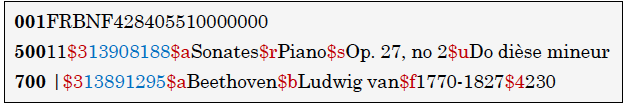
\includegraphics[width=10cm]{img/marc-exmpl-simple.png}
  \caption{An excerpt of a UNIMARC record.}
  \label{fig:unimarc}
\end{figure}

We have developed an open source prototype that allows for the automatic conversion of bibliographic records given in UNI- or INTERMARC to RDF\footnote{\url{https://github.com/DOREMUS-ANR/marc2rdf}}. One of the particularities of this converter is that it implements the DOREMUS model. The conversion process relies on explicit expert-defined transfer rules (or mappings) that indicate where in the MARC file to look for what kind of information, providing its corresponding property path in the model as well as useful examples that illustrate each transfer rule, as shown in Fig.~\ref{fig:mappings}. The mapping rules reflect the practices of each institution and therefore a mapping table per institution has been provided by the experts. We have used the DOREMUS properties to name the extracted relations (as for example \texttt{mus:U12$\_$has$\_$genre}\footnote{The \texttt{mus} prefix refers to \url{http://data.deremus.org/ontology/}}, labeling the property describing the genre of a music work). The resources are identified by URIs that use the corresponding DOREMUS class labels in their names (as for example \url{http://data/doremus.org/expression/UUID} identifying in an unique manner an instance of the FRBRoo class \texttt{Expression}).

\begin{figure}
  \centering
  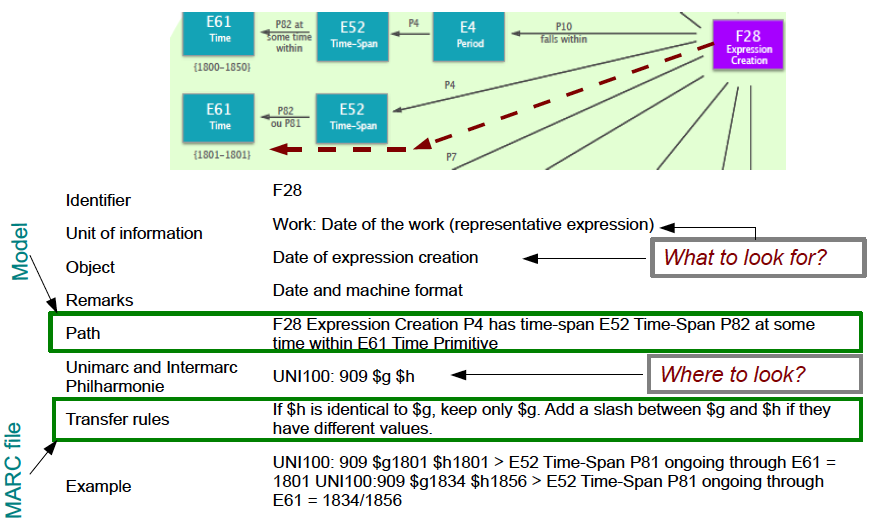
\includegraphics[width=11cm]{img/mapping-rules.png}
  \caption{Example of mapping rules regarding the timespan of the composition of a work.}
  \label{fig:mappings}
\end{figure}

Often, the RDF data that we extract will contain string literal values, such as genres ({\it sonata}), instruments ({\it piano}), tonalities ({\it D-major}) and other. As introduced above, these values are controlled by specific vocabularies, such as the MIMO vocabulary\footnote{\url{http://www.mimo-international.com/vocabulary.html}} describing musical instruments. Therefore, our data conversion methods include an automatic mapping of string literals to URIs coming from controlled vocabularies. We have used the {\tt string2uri} mapper, relying on various string matching techniques\footnote{\url{https://github.com/ThibWeb/stringtouri}}.

An example of a converted MARC record is given in Fig. \ref{}. %Not sure we need an example.

%%%%%%%%%%%%%%%%%%%%%%%%%%%%%%%%%%%%%%%%%%%%%%%%%%%%%%%%%%%%%
%%%  3. OVERTURE: an Exploratory Search Engine for Music  %%%
%%%%%%%%%%%%%%%%%%%%%%%%%%%%%%%%%%%%%%%%%%%%%%%%%%%%%%%%%%%%%

\section{OVERTURE: an Exploratory Search Engine for Music}
\label{sec:overture}



%\begin{figure}
%  \centering
%  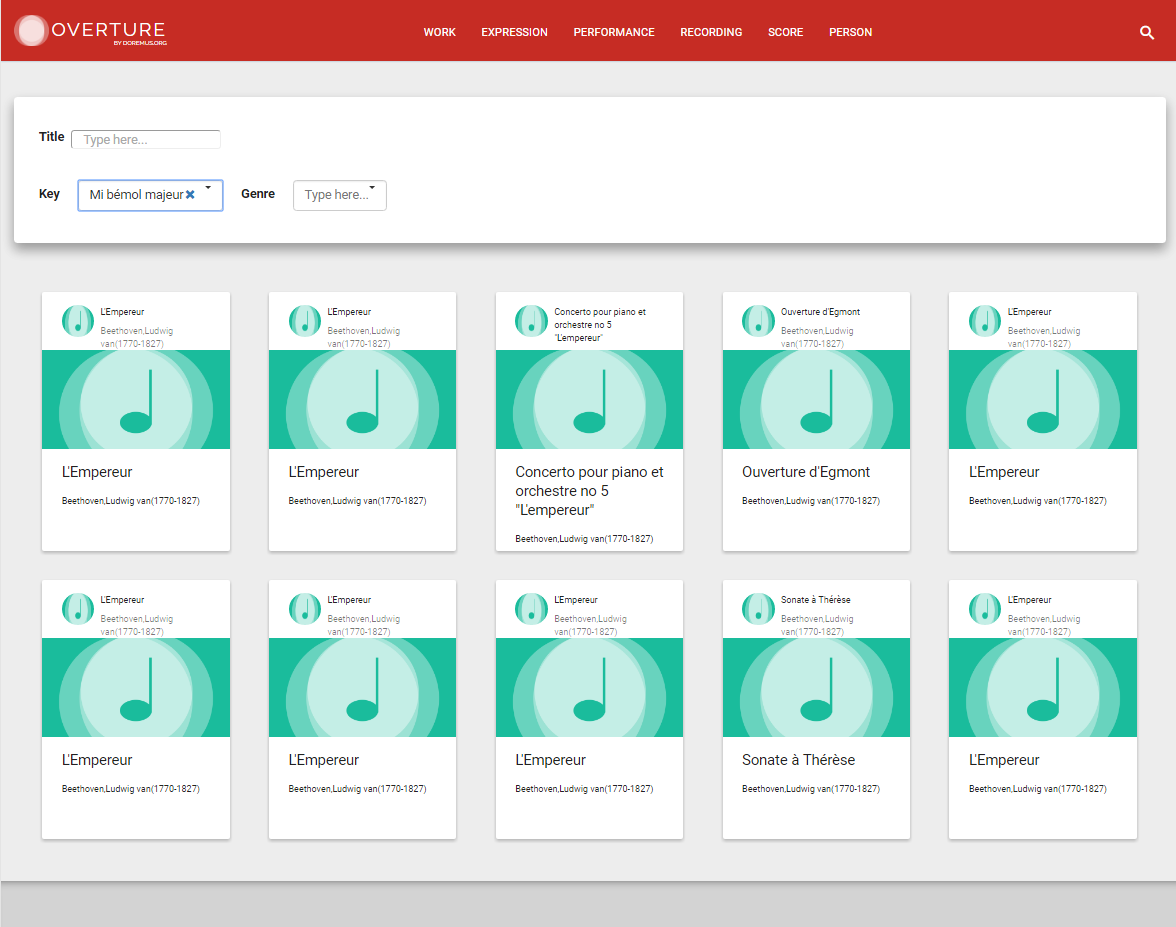
\includegraphics[width=11cm]{img/overture-list.png}
%  \caption{Overture interface: the search form and results.}
%  \label{fig:overture-list}
%\end{figure}

\begin{figure}
  \centering
  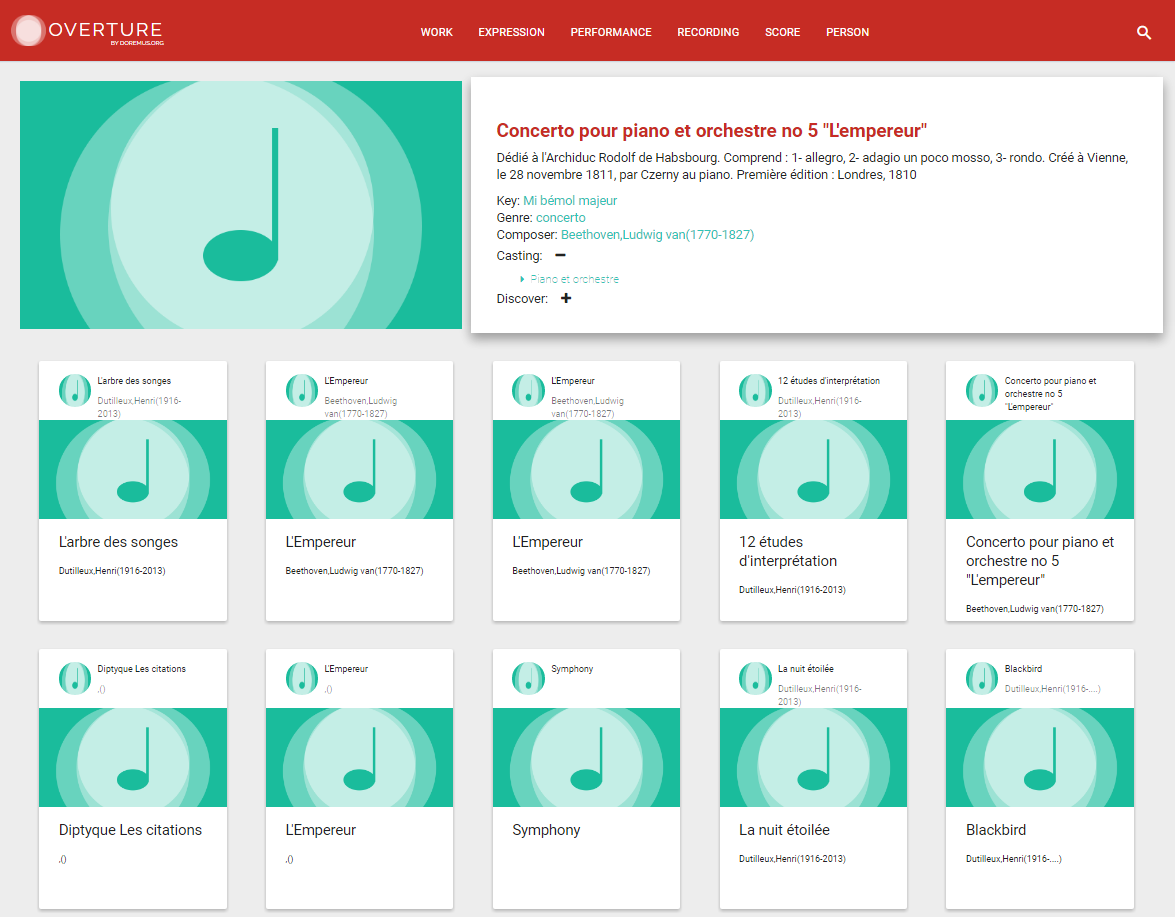
\includegraphics[width=11cm]{img/overture-detail.png}
  \caption{Overture: Browsing Expression ...}
  \label{fig:overture-detail}
\end{figure}

OVERTURE (Ontology-driVen Exploration and Recommendation of mUsical REcords) has been developed as a modern web application. Its Node.JS server sits in front of a Virtuoso repository, in which we store the results of the conversion, and retrieves the information from it through SPARQL queries.

Figure \ref{fig:overture-detail} shows the user interfaces realized with AngularJS. On top, a navigation bar directs the user towards one of the main concepts in the DOREMUS model (Work, Expression, Performance, Recording, Score, Person), that become distinct sections of the application. Inside each section, the user can filter the list of records shown in a class-specific and advanced search form. In this way, (s)he can search a performance by choosing a particular location,a performer, or an expression by selecting the musical key, the genre or by writing its title. From these parameters, the server generates the SPARQL query that matches the user information need (Figure \ref{fig:sparql}). 

Clicking on a result, more details are shown like the information about the composer, the casting and a longer descriptive note. Beside it, a selection of different expressions is shown; in future, this selection will contain related expressions, selected through a reccomandation algorithm.

\begin{figure}
\centering
\begin{verbatim}
SELECT ?expressions ?title
WHERE {
    ?expressions a  frbroo:F22_Self-Contained_Expression ;
        cidoc:P102_has_title ?title .
        mus:U12_has_genre <http://data.doremus.org/vocabulary/genre/si>
}
\end{verbatim}
\caption{Overture: A simplified example of the SPARQL query that extracts the titles of expressions that have the genre "symphony".}
\label{fig:sparql}
\end{figure}

% TODO link to demo video

%%%%%%%%%%%%%%%%%%%%%%%%%%%%%%%%%%%%%%%
%%%  4. Conclusion and Future Work  %%%
%%%%%%%%%%%%%%%%%%%%%%%%%%%%%%%%%%%%%%%

\section{Conclusion and Future Work}
\label{sec:conclusion}
We are currently working on the development of connectors for music works, allowing for the automatic interlinking of equivalent resources across datasets of different bibliographical agencies. Our first test with the SILK \cite{jentzsch2010silk} and LIMES \cite{ngomo2011limes} tools confirm our initial hypothesis that new methods, specific to the music field, need to be proposed, able to handle the high heterogeneity of these datasets. In particular, our first tests show that special attention has to be payed to multilingual descriptions of works, as well as to significant differences in lexical descriptions of music titles. Descriptive heterogeneities (level of detail, amount of information available) also appear to be hard to handle by the existing general purpose off-the-shelf linking tools. We plan to combine expert heuristics with an automatic heterogeneity centered data linking approach. Finally, the developed connectors will be integrated to the OVERTURE application, allowing for the automatic navigation from one dataset to another bringing to the user the richness of several connected datasets.

Recommendaiton ?

\section*{Acknowledgments}
This work has been partially supported by the French National Research Agency (ANR) within the DOREMUS Project, under grant number ANR-14-CE24-0020.

\bibliographystyle{abbrv}
\bibliography{bib-doremus}

\end{document}
